% =====================================================================
%  Chapter 2 — What "Protect the Principal" Means in Arithmetic
% =====================================================================

\chapter{What ``Protect the Principal'' Means in Arithmetic}
\label{ch:principal}

A portfolio cannot protect its principal. Every portfolio that has ever
existed has, at some point, been worth less than it was. What a portfolio
can do is make the set of outcomes it produces survivable by the person
holding it, and that is a statement about a distribution, not about a
minimum.

This chapter converts the owner's phrase into three computable quantities and
then asks how much they cost. The answer, which is uncomfortable and
instructive, is that principal protection is not free and is not cheap: every
unit of drawdown reduction is bought with a measurable slice of expected
return, and the exchange rate depends on which part of the distribution the
investor cares about.

\section{The three quantities}

Given a monthly total-return series \(r_t\) for the portfolio, the book
computes three numbers and no others when it makes a protection claim.

\paragraph{The maximum drawdown}
\begin{equation}
\mathrm{DD}_{\max} = \min_{0 \le t \le T}
\left( \frac{W_t}{\max_{0 \le s \le t} W_s} - 1 \right),
\qquad
W_t = \prod_{i=1}^{t}(1+r_i).
\end{equation}
The drawdown is measured from the running peak, which is the right
reference: an investor's experience of loss is relative to the best recent
state of their own account, not to their initial deposit. This is the
number that produces the visceral response, and for a single investor whose
capital is also their salary buffer, it is often the binding constraint.

\paragraph{The time to recovery}
\begin{equation}
T_{\mathrm{rec}} = \min\left\{ k \ge 1 :
W_{t+k} \ge \max_{0 \le s \le t} W_s \ \text{ for all } t \text{ with a
prior drawdown}\right\},
\end{equation}
computed from each drawdown trough as the number of months until the
portfolio regains its prior peak. Time to recovery is the quantity that
separates a drawdown from a catastrophe. A 30 per cent drawdown recovered in
eighteen months is a bad year; a 30 per cent drawdown that takes nine
years to recover is a different instrument entirely, and it is the
instrument that breaks a saver who stops saving.

\paragraph{The worst twelve months}
\begin{equation}
R_{12}^{\mathrm{worst}} = \min_{t}\left[
\prod_{i=t}^{t+11}(1+r_i) - 1 \right].
\end{equation}
The worst rolling twelve-month outcome is the number the investor should
actually plan around, because the calendar year is an artefact of the
investor's own habit of checking a statement once a year. It is also the
quantity that determines whether a withdrawal rate is safe.

\begin{takeaway}[The protection contract]
A protection claim in this book means a stated pair of numbers: a maximum
drawdown and the time to its recovery. A third number, the worst rolling
twelve-month return, is carried alongside them because it, and not the
calendar year, is what a saver's plan has to survive.
\end{takeaway}

\section{Why the arithmetic mean is the wrong summary}

There is an identity that governs all of this and that most performance
discussions avoid. If a portfolio's monthly returns have arithmetic mean
\(\mu\) and variance \(\sigma^2\), then over \(T\) months the geometric
mean is

\begin{equation}
g = \left[\prod_{t=1}^{T}(1+r_t)\right]^{1/T}
   \approx \exp\left(\mu - \frac{1}{2}\sigma^2\right)
\end{equation}
when the returns are small, and the approximation is the one that matters
here. The gap between the arithmetic and geometric means is \(\sigma^2/2\)
per period: at an annual volatility of ten per cent, the geometric mean is
roughly five percentage points a year below the arithmetic mean. At fifteen
per cent it is roughly eleven.

\begin{figure}[!htbp]
\centering
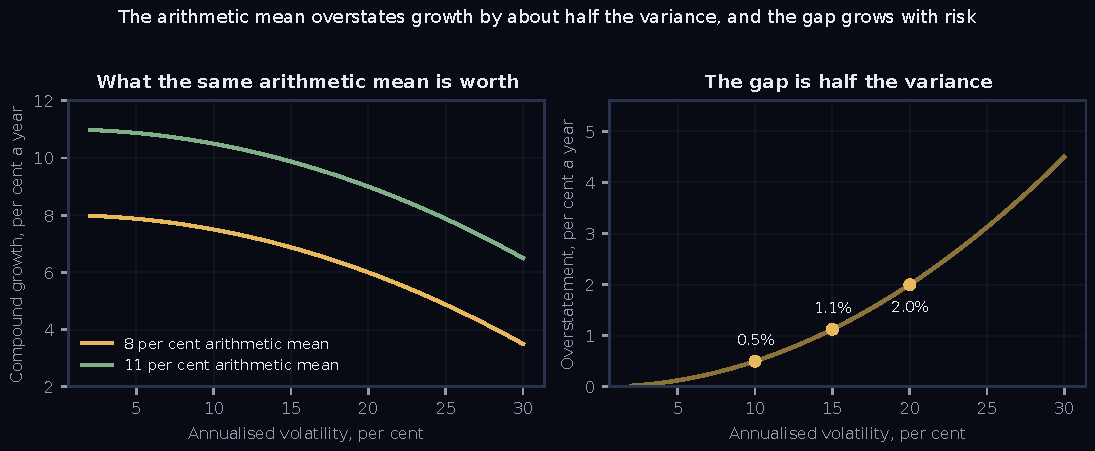
\includegraphics[width=\textwidth]{../figures/fig_arith_geom.pdf}
\caption{The arithmetic and geometric means of the same return series, and
the volatility penalty between them. The penalty is \(\sigma^2/2\) per
period and it grows quadratically: the difference between an arithmetic and
a geometric claim is a statement about volatility, not about skill.}
\label{fig:arith-geom}
\end{figure}

\figref{fig:arith-geom} is the reason the book refuses to argue in terms of
the arithmetic mean. An arithmetic claim of ``one per cent more per year''
is worth less than it sounds whenever it is accompanied by higher
volatility, and a geometric claim of the same magnitude is worth more than
it sounds. Since the owner asked for money, and money is compounded, the
geometric mean is the object.

The same identity explains why volatility reduction can be worth a great
deal to a saver even when it costs arithmetic return. If a modification
lowers volatility from fifteen to eleven per cent, it buys back about
\((0.15^2 - 0.11^2)/2 = 5.2\) percentage points a year in geometric terms.
If it costs one point of arithmetic return, it is worth doing. If it costs
four, it is not. Every design decision in Part V of this book is, explicitly,
a bet on which side of that trade it falls.

\section{The cost of protection, measured on this portfolio}

The system's own record lets this be measured rather than asserted. Part VI
reports four portfolios over the same window: the stated strategic policy
alone; the policy with the model's tilt; the policy with the risk
governor; and the whole system. The governor is the protection layer, and
its cost is the difference between its compound growth rate and the
policy's.

The number that matters is not the growth rate. It is the pair: what the
drawdown was, and what the growth rate was, for the same portfolio. A
reader who believes the system's own numbers should note that the
protection this book buys is a \emph{reduction in the depth and duration of
the worst episode}, not the elimination of loss, and it is bought at a
stated price in compound return.

\begin{commonmyths}
\item \textbf{Myth: ``Capital preservation and growth are opposites.''}
Fact: they are opposites only if the investor is risk-neutral and
myopic. Because the geometric mean is \(\mu - \sigma^2/2\), a
volatility reduction of a given size is worth a given amount of compound
return, and the two can be traded. The trade is the whole subject of
Part V.
\item \textbf{Myth: ``Stop-losses protect the principal.''}
Fact: a stop-loss sells at the bottom of a loss and prevents the recovery
that follows it. It converts a temporary loss into a permanent one and
raises the variance of the outcome it was meant to reduce. The book's
governor acts on \emph{exposure}, not on orders, which is a different
mechanism entirely.
\item \textbf{Myth: ``Diversification is the protection.''}
Fact: diversification reduces the volatility of the average holding but
does nothing about the sequence in which returns arrive, which is what
actually kills a saver. That gap is the subject of Chapter 7.
\end{commonmyths}

\section{The three numbers a saver should write down before starting}

Before any model, any factor, any allocation: the reader should be able to
state the maximum drawdown they will not abandon the strategy for, the
number of years they can wait for a recovery, and the annual withdrawal
their plan depends on. Those three numbers define the feasible set of
portfolios, and they are inputs to the system, not outputs of it. A
portfolio whose drawdown exceeds the first number cannot be held by someone
who means it; no amount of expected return compensates, because the
investor's behaviour under a drawdown is not a decision variable that the
portfolio controls.

This is the deep reason the book puts a stated strategic allocation outside
the reach of the machine. The strategic allocation determines the drawdown
the investor must be able to sit through, and that is a fact about the
investor's circumstances --- their income, their age, their willingness to
stop saving --- and not something a learning algorithm can discover from a
price series.

\begin{keytakeaways}
\item Protection is three numbers: maximum drawdown, time to recovery, and
the worst rolling twelve-month return. It is never a minimum.
\item The gap between the arithmetic and the geometric mean is \(\sigma^2/2\)
per period; volatility reduction is therefore a source of compound return,
not a concession.
\item The protection layer of this book has a stated price, paid in compound
return, and the price is reported in Part VI rather than assumed.
\item The strategic allocation is set from the investor's circumstances, not
from the data, and the machine is not permitted to set it.
\end{keytakeaways}
